
\section{Methods}             % chapter 2
\subsection{Search}     % section 2.1
In order to perform reputation management, relevant opinions must be found. Twitter provides the ability to search for specific keywords \cite{Golovchinsky_makingsense}, partially solving this problem. However, while their in-memory search solution is fast, it is also limited to the last 8 days. We store search results in a relational database\footnote{Our choice of RDBMS is MySQL.}, which is also queried when an analysis is performed. MySQL offers full-text search indexes, which sort results based on a TF-IDF measure \cite{suchal2010full}. Since only a subset of found tweets is sampled\footnote{Up to 100 tweets per hour.}, it can occur that the database search also returns tweets stored for another query, slightly increasing recall.

All results are regarded as relevant, whether they are retrieved directly through Twitter Search, or found by the database text search. Since tweets are limited in length, a relevance score based on term frequency and document frequency would not yield useful information; thus, tweets are not sorted by search relevance.


\subsection{Tweet Retrieval}	% section 2.2 
The first step before being able to do any kind of analysis is retrieving data about the tweets. Besides the actual tweet text, information about the users that posted the tweets and properties such as the number of retweets, followers and favourites are required.

Twitter offers access to most of its functionalities through a REST API. Rather than writing a Java/REST connector, the open source twitter4j library was used. Although it is not an official library, it provides direct access to the data through Java function calls. On top of this library another layer, specific for the current use-case, was added.

One problem that quickly surfaced was the rate limit imposed by the API. The program can only do 150 calls per hour, when not authenticated, and 350 otherwise. In the case of the tweet data this issue was solved by employing a common strategy in such situations - caching. By extending the classes in the twitter4j library, the methods work regardless of where the actual data is coming from - be it database or twitter search. However, in the case of the user data, this limitation meant not being able to do a PageRank implementation on a user graph. Relevant user information (number of followers, friends and tweets) was therefore cached as well, in order to decrease the potentially higher number of requests per search query.

\subsection{Sentiment Analysis}	% section 2.3

\subsubsection{Preprocessing}       % subsection 2.3.1

Prior to performing the sentiment analysis of the tweets, it is common to use preprocessing techniques to achieve better results with less noise. For this implementation, two main techniques have been used: annotation and URL removal,  and elimination of repeated characters inside the tweet. 

Twitter users often use an informal way to express their feelings. It is common practise to express our enthusiasm for something, by repeating some characters e.g "greeeeeaaaat product!", "So aweeesome!". Thus, there is a great need to eliminate these characters without loss of information, e.g look can miss-mapped to lok. As a result we assigned the repeated characters to a double character representation, i.e. greeaaaaat mapped to greeaat.
In addition to this and after some experiments we realized that in tweets, often references and links are used, such as 

\begin{quotation}
"@someone Google is awesome.check this www.in.gr" 
\end{quotation}
 
This adds additional noise; such references are therefore removed prior to the actual sentiment analysis.


\subsubsection{Tokenization}       % subsection 2.3.1

Before analysing the tweets, tokenization techniques have been applied. Initially, a simple tokenization that split the text using whitespaces as delimiters was used. In this process, words and punctuation can constitute a token. 
This tokenization is restricted and needed improvements to handle punctuation. For the final tokenizer, the StandardTokenizer class of Lucene \cite{hatcher2004lucene} is used\footnote{Apache, http://lucene.apache.org/}. This tokenizer splits words at punctuation characters, removing punctuation, and at hyphens; unless there is a number in the token, in which case the whole token is interpreted as a product number and is not split. With this tokenizer it is also possible to recognize email addresses and internet host names as one token.


\subsubsection{Lexicon}

Once tweets about the company we are searching for have been retrieved, they must be analysed to determine their polarity. 
Three labels are used for the tweets: negative, neutral and positive. A neutral tweet is defined as a tweet with a sentiment score that approaches 0. 

To perform this analysis, a sentiment lexicon is used. The lexicon is made of sentiment words associated with a score, for example (good: +1), (bad: -1), (like: +1), (hate: -2).
Using the lexicon is quite easy; one just needs to sum up the score of each token to have the overall sentiment score of a tweet. 
However, this method can be improved upon using some heuristics. 

The first thing to take into account is the negations' problem. To deal with this problem, negations were added in the database and when a negation is found in a sentence, 
scores of the two following words are reversed; multiplying them by -1. For example "This is not good" will give a score:
\begin{eqnarray}
	(-1) \cdot (+1) & = & -1
\end{eqnarray}

In the same way, some modifiers were added to our analysis. Modifiers are words like "really", "very" or "quite". 
All these words modify the sentiment score of the following word, multiplying it by a factor proportional to the strength of the modifier. For example, "very" will multiply by 2, whereas "quite" will multiply by 0.5.

Then it is also important to deal with sentences like "I love company A, but I hate company B". 
For this, the notion of distance was added to the analysis. The distance will increase the score of sentiment words close to the name of the company and reduce 
the score of sentiment words far away. A Gaussian distribution is used with a maximum distance of 4; this means that sentiment words that are far from the name 
of the company (more than 4 words between them) are not taken into account.

\subsection{PageRank}
Besides making sentiment analysis on tweet content, it is important to use some kind of static / authoritative quality measure to assign importance to the tweets themselves. For this purpose, certain tweet features were utilized. A tweet's "importance" / "effectiveness" (regardless of its sentimental value) is determined through the following: how many times a tweet is retweeted and if it is favorited, how many followers, friends and other tweets of the author of the tweet exist. Using the information available on the web about the maximum of such numbers (for instance, no one has more than 25 million followers to the date), using log of the features and a simple linear mixture, we get a single number. This number is then used in conjunction with the sentiment score.

Please note that "PageRank" is kind of a misnomer in this case, since we could not apply the original pageranking algorithm due to technical limitations of Twitter API (as described in Tweet retrieval part above). Since we do not have access to the whole graph, we tried to solve the problem with a more limited set of importance indicating features.

\subsection{Naive Bayes}
In order to assign an additional score based on previous data, the naive bayes model has been used. Based on the algorithm provided by Weka\footnote{Weka, http://www.cs.waikato.ac.nz/ml/weka/}, we used previous hand-classified data provided by Sanders Analytics \cite{sandersanalytics} . The format of this data can be seen in table \ref{table:dataformat}. From every tweet we extract its content and transform it into a feature vector by using the Weka Filter StringToWordVector. Afterwards, we train the model with the extracted annotated data and serialize it in order to classify new tweets based on their content. However, a very important concept in machine learning and data mining is the overfitting issue occurring when a model is too perfectly fit to a limited set of training data points. For this reason we used the 10 folds cross-validation offered by Weka.

\subsection{User Interface}
Reputation is a relatively new, and as of yet unknown field. Most users will be relatively new to reputation monitoring tools, and have little experience interacting with them. It is therefore beneficial to keep the design as simple and self explanatory as possible, while maintaining the essential functionality. The first step is thus to perform a functional analysis to define the user needs:

\begin{itemize}
	\item The user must be able to input the brand or term whose reputation he wants to monitor.
	\item In a clear way, the overall result must be returned: what is the general, time independent sentiment?
	\item Did this sentiment change over time?
	\item Optional: what data is this based on?
\end{itemize}


\subsubsection{Search Input}
Initially, the search input was designed to allow the user a great degree of control and customization; the use of boolean operators and query expansion would enable a fine-tuned search for a specific subset of terms, related to the intentional query. In practice, this was abandoned for two reasons:

\begin{enumerate}
	\item A simple word specific search would already yield a great many results, even for relatively  unknown terms. This excess of data precludes the use of query expansion and thesaurus lookups.
	\item Only trained users would likely use this specific functionality \cite{jansen2000real}. For all but the most experienced users, excess functionality would needlessly complicate the application.
\end{enumerate}

Eliminating all non-essential features yielded the search input form in figure \ref{fig:gui_search}. The user is presented with a single text input field and a single button. The only distracting elements are the status bar at the bottom (which provides real time information on the analysis progress) and a tab bar, enabling a user to switch to previous search results.

\begin{figure}[h]
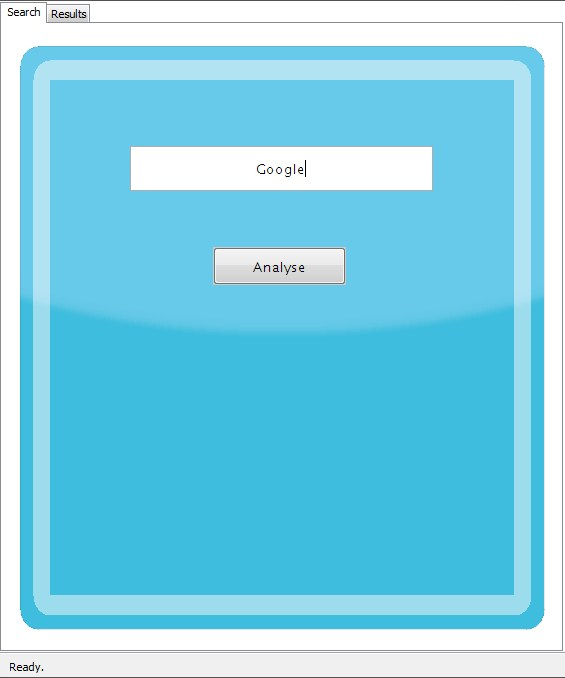
\includegraphics[width=0.5\columnwidth]{./images/search_input.jpg}
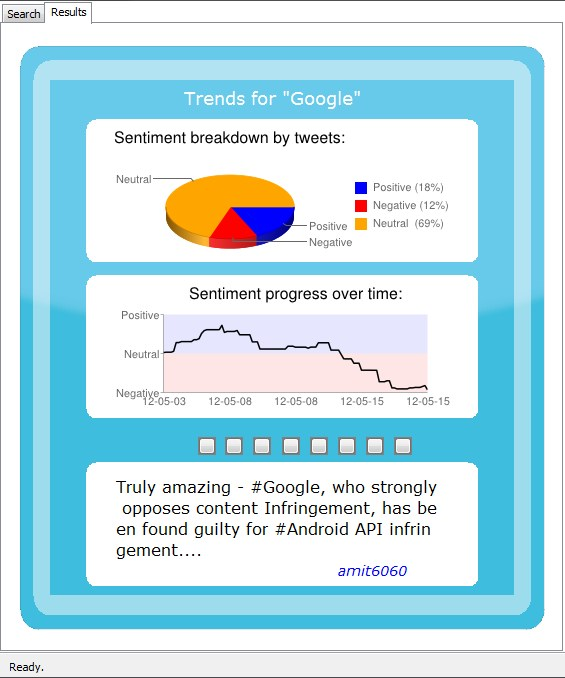
\includegraphics[width=0.5\columnwidth]{./images/search_results.jpg}
\caption{Search input (left) and results (right).}
\label{fig:gui_search}
\end{figure}

\subsubsection{Search Results}
The functional analysis yielded a need to visualize the overall reputation for a given query. To this end, a break-down of positive, negative and neutral tweets is displayed as pie chart. The Google Charts API\footnote{https://developers.google.com/chart/} enables simple creation and insertion of such charts into any application. From this overview, a user can deduce at a glance whether people post more positive or more negative opinions. These results are integrated over all time, and may therefore not reflect the current opinion.

To provide time dependent information, a second graph is used to display the cumulative reputation over time. Each tweet is considered a single instance, and its sentiment score is added to the sum of sentiment scores up to that point in time. No time dependent binning of tweets is performed: due to the irregular nature of tweets, this would force unacceptably large bin sizes. A net result of this is that the effective resolution of the graph increases during moments when more tweets are posted. An example of this is illustrated in figure \ref{fig:gui_search}.

Lastly, a list of top-ranked tweets is provided. By clicking on any of the square buttons, a top-sentiment tweet can be viewed. This enables the user to know what it is exactly that the most prominent advocates of the search query say about it.








